\documentclass[11pt,a4paper]{article}% 文档格式
\usepackage{ctex,hyperref}% 输出汉字
\usepackage{times}% 英文使用Times New Roman
\usepackage{amsmath, amsthm, amssymb, appendix, bm, graphicx, hyperref, mathrsfs, float,subfigure,booktabs,tabularx,longtable,geometry,pdfpages}
%\usepackage{fancyhdr}	% 用于更改默认的页眉页脚格式
\usepackage{listings}  % 用于插入代码
\usepackage{xcolor}  % 用于设置颜色
\usepackage{caption}
\usepackage{booktabs,multirow}
\usepackage{lipsum} % 用于生成虚拟文本的包
% 将目录标题居中
\renewcommand{\contentsname}{\centering Content}
\renewcommand\contentsname{Content}
\renewcommand{\figurename}{Figure}
\renewcommand{\tablename}{Table}
\captionsetup{labelformat=default,labelsep=space} %去除冒号

\title{\textbf{\Huge Simulation Report of Barrier Gate}}
\date{}

\graphicspath{{img/}}
\bibliographystyle{plain}

\begin{document}

\begin{figure}
    \centering
    
\includegraphics[scale=1.2]{SJTU}
\end{figure}

\maketitle

\begin{table}[b]
    \centering
    \begin{tabular}{>{\bfseries}c>{\centering\arraybackslash}p{5cm}}
        Name: & Chen LeKai \\
        \cline{2-2}
        ID: & 521020910180 \\
        \cline{2-2}
        Date: &  2024.4.23\\
        \cline{2-2}
    \end{tabular}
\end{table}

\thispagestyle{empty}

\newpage
\pagenumbering{Roman}
\setcounter{page}{1}
\tableofcontents

\newpage
\pagenumbering{arabic}
\setcounter{page}{1}

\newpage
\setcounter{page}{1}
\section{Project Background}
The barrier gate is quite common in the car park. In this project, we hope to model the barrier gate by using a DC motor and design a closed-loop controller to make the barrier gate more stable, accurate and safe in operation.
Before the physical design, we explore the control principle, characteristics and control mode of the DC motor through Simulink simulation firstly, design the appropriate control algorithm and carry out simulation for verification. Through the simulation, we can find out the parameters of the controller more quickly and intuitively, which provides reference for the future physical design.

\begin{figure}[H]
    \centering
    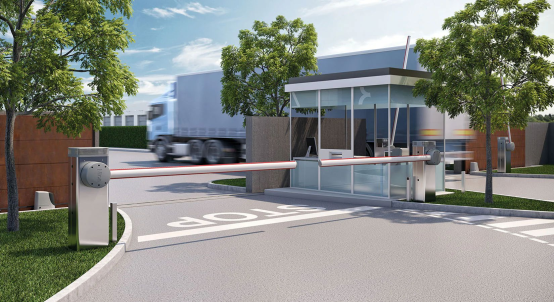
\includegraphics[width=0.8\textwidth]{Abarriergate}
    \caption{A barrier gate}
    \label{fig:Abarriergate}
\end{figure}

\newpage
\section{DC motor simulation model}
According to the actual motor parameters of the project, we establish the DC motor model in Simulink, and its specific parameters are shown in the following table.
\begin{table}[H]
    \centering
    \begin{tabularx}{\textwidth}{>{\centering\arraybackslash}X>{\centering\arraybackslash}X>{\centering\arraybackslash}X>{\centering\arraybackslash}X}
        \toprule
        Parameter & Value & Unit & Description \\
        \midrule
        Feild Type & / & / & Permanent magnet \\
        Inductance & $12 \times 10^{-6}$ & H & Inductance \\
        No-load Speed & 12 & rpm & / \\
        Rated Speed & 9 & rpm & / \\
        Rated Load & 5.4 & W & / \\
        Supply Voltage & 12 & V & / \\
        No-load Current & 120 & mA & / \\
        \bottomrule
    \end{tabularx}
\end{table}



\section{Closed-loop controller design}
The controller is the brain of the system. It receives the error signal (for closed-loop control) as its input, and develops an output signal that causes the controlled variable to become the value specified by the setpoint. For the barrier gate, we can simply set the running time of the motor to open and close the barrie gate.
However, considering that during the operation of the equipment, it is difficult to avoid interference from environmental factors, such as sudden voltage jumps, air resistance, internal friction of the motor and its own inertia. It is difficult to realise the position and speed accuracy of the barrier gate by simple open-loop controller. The inaccuracy in position may lead to problems such as inaccurate running interval and collision between the bar and environmental objects after a long time of operation.
Therefore, we need to design a closed-loop controller that can resist environmental interference to a certain extent, and adjust the control signals by detecting the running state of the barrier gate, so that the target parameters(position, speed) are always in line with the setpoint, thus achieving the stable operation of the barrier gate. In the following sections, we will introduce the design of several kinds of closed-loop controllers based on PID controllers.
In addition, we will also introduce the tuning process of these controllers and their control effect in the following sections.

\subsection{Speed PID controller}
\begin{figure}[H]
    \centering
    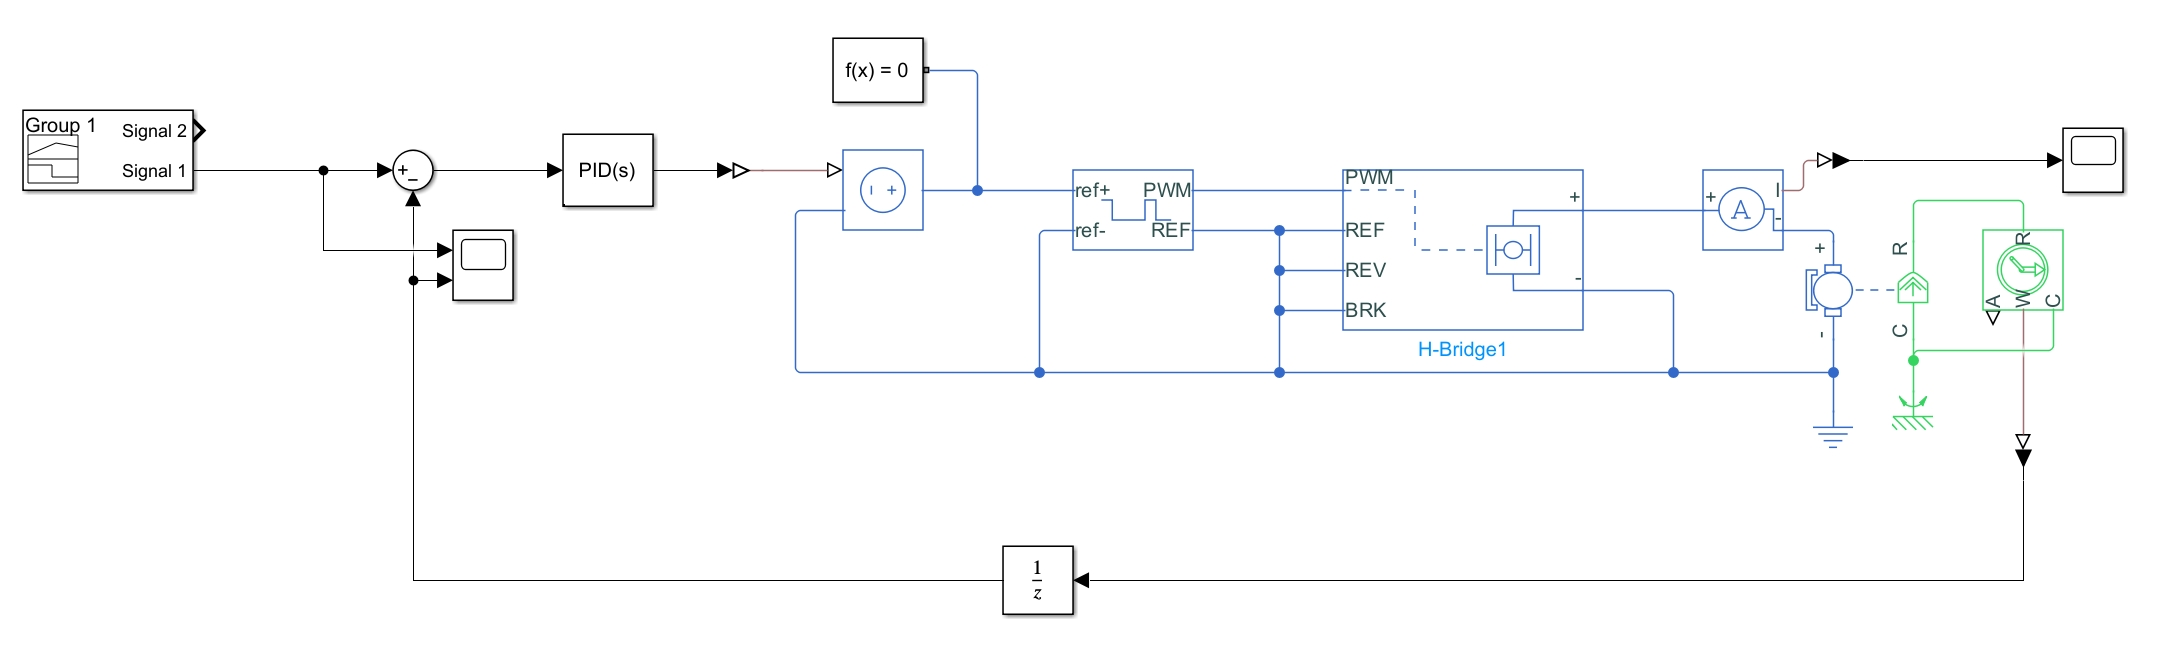
\includegraphics[width=1\textwidth]{controller1}
    \caption{Speed PID controller}
    \label{controller1}
\end{figure}
As it shown in the figure \ref{controller1},The speed control signal is passed through the controller to the controlled power supply, which is used to generate a PWM voltage signal with a duty cycle proportional to the voltage of power supply.And then passed through the H-Bridge to drive the motor.
Since we are simulating a single-step (opening or closing the barrier gate) operation here, it is sufficient to ground all the other control signals of the H-Bridge except for the PWM signal.

Rotation motion sensor is used to detects the motor's speed (W), position (A) and other information. In the speed PID controller, we only use the speed as the feedback variable.
The actual speed is fed back and compared with the setpoint, and the calculated error signal is used as the input of the PID controller. 
Considering that in the actual microcontroller system, PID control is often carried out in the form of timed interrupt, and the feedback signal is not collected continuously, a delayer is added to the feedback signal to simulate the process of sampling and updating the error signal at regular intervals.
Here, the sampling period is set as

\begin{equation}
    T_s = 0.02s
\end{equation}

\subsection{Position and velocity parallel PID controller}
\begin{figure}[H]
    \centering
    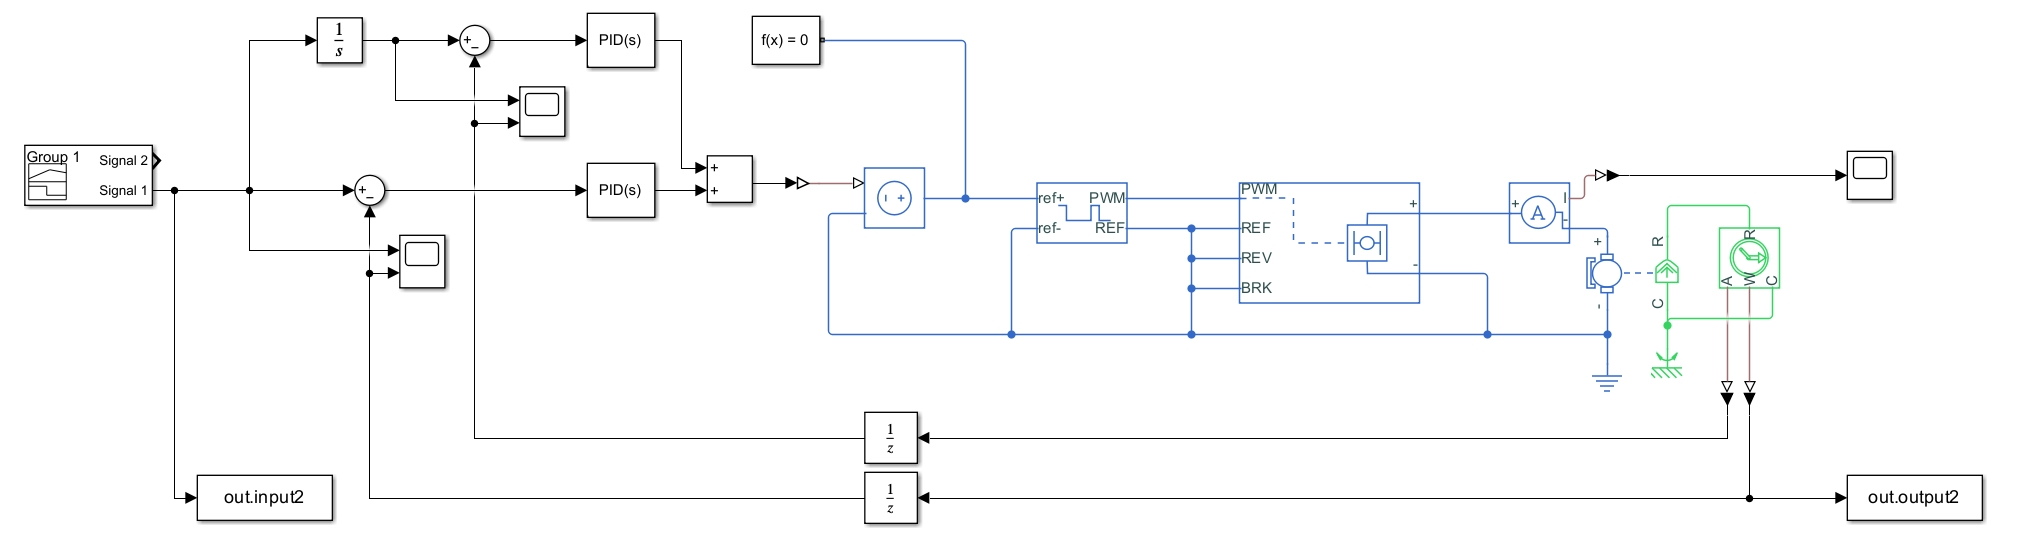
\includegraphics[width=1\textwidth]{controller2}
    \caption{Position and velocity parallel PID controller}
    \label{controller2}
\end{figure}
As it shown in the figure \ref{controller2},We firstly integrate the velocity control signal to obtain the real-time position control signal, and secondly, 
, we utilise the position signal output from the ideal rotational motion sensor, and similarly we take the collected position information for
feedback and compare it with the position control signal to get the position error, and then sum the velocity error and position error as the input signal to the PID controller.


The controller designed in this way takes two factors into account simultaneously, which can more comprehensively reflect the characteristics of the control signal. The biggest problem with a simple speed controller is that there may inevitably be errors in the speed of the DC motor, resulting in the angle of each displacement being difficult to accurately reach ninety degrees. In the actual scenario of a parking lot, after multiple reciprocating movements of the bar, significant drift in its range of motion will occur, which is obviously unacceptable. By incorporating the position error signal, it is possible to better reflect the problem of bar position deviation and correct it.

\subsection{Position, speed, current serial PID controller}
\begin{figure}[H]
    \centering
    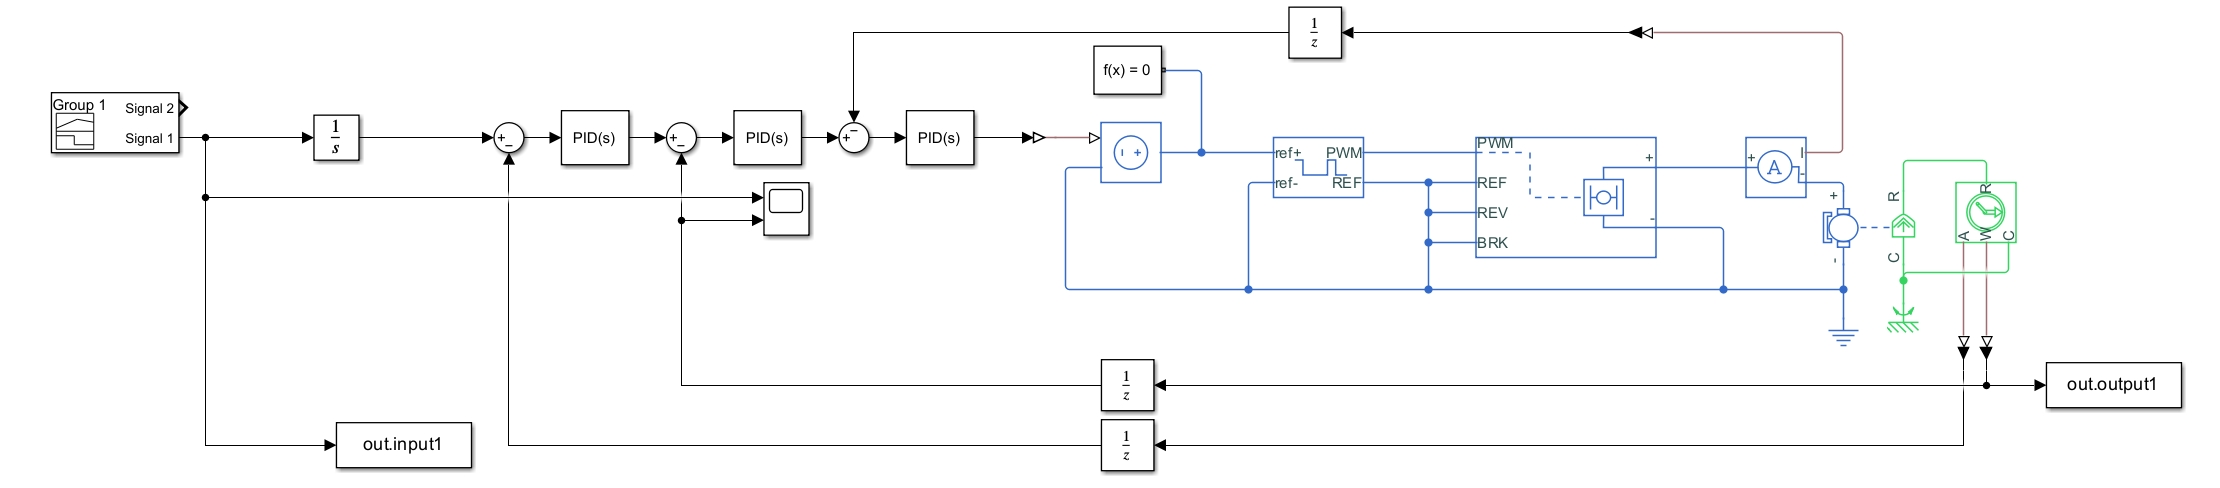
\includegraphics[width=1\textwidth]{controller3}
    \caption{Position, speed, current serial PID controller}
    \label{controller3}
\end{figure}

In practical control systems, based on engineering experience, the use of a serial PID controller for position, velocity, and current control has shown excellent performance. Here, we also consider it as a design of a closed-loop controller. Its principle is similar to that of a parallel PID controller for position and velocity, but with the addition of a current signal in the input to reflect the motor torque. This helps to better reflect the actual operating state of the motor. Furthermore, the parallel inputs are converted to serial inputs, with the error of position serving as the reference signal for velocity comparison, and the error of velocity serving as the reference signal for current comparison

Here, three PID controllers are employed, which makes tuning more complex. According to engineering experience, the bandwidth of the current loop is the widest, followed by the velocity loop, and the position loop has the narrowest bandwidth. Therefore, we can start by tuning the current loop, then proceed to tune the velocity loop, and finally tune the position loop. After tuning each PID controller individually, they are then connected in series to achieve the best control performance.

\newpage
\section{Motion Profile}
Motion profile is a set of reference trajectories that define the desired motion of the system. It is used to generate
the reference signal for the controller. In this project, we will use two different motion profile to control the barrier gate.
The first motion profile is Trapezoidal motion profile, which is a common motion profile used in industry. The second motion
profile is S-curve motion profile, which is a more smooth and natural motion profile. The two motion profiles are shown below.
\begin{figure}[H]
    \centering
    \subfigure[Trapezoidal motion profile]{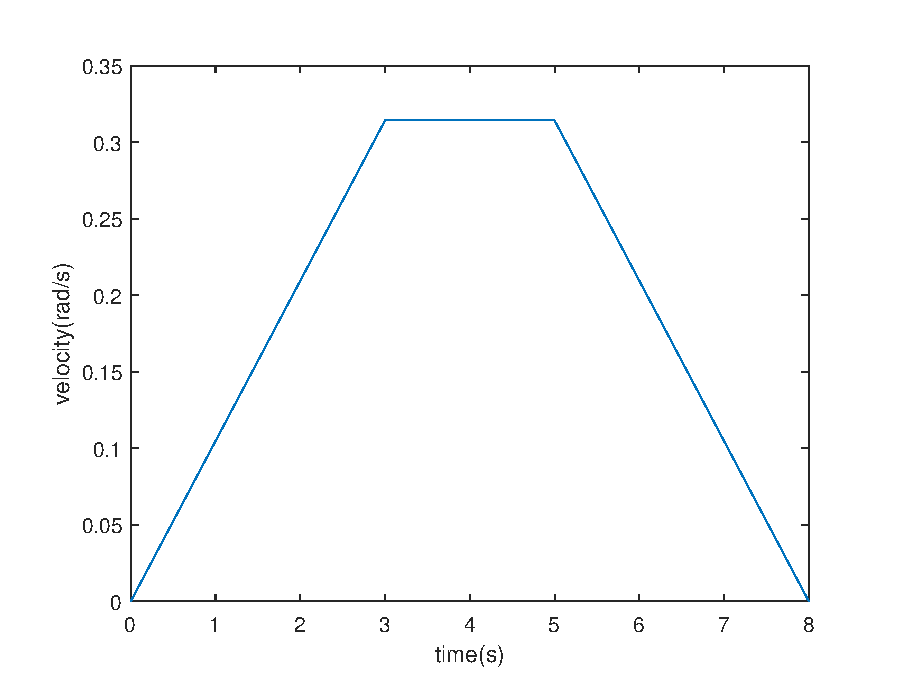
\includegraphics[width=0.45\textwidth]{TrapezoidalCurve}}
    \subfigure[S-curve motion profile]{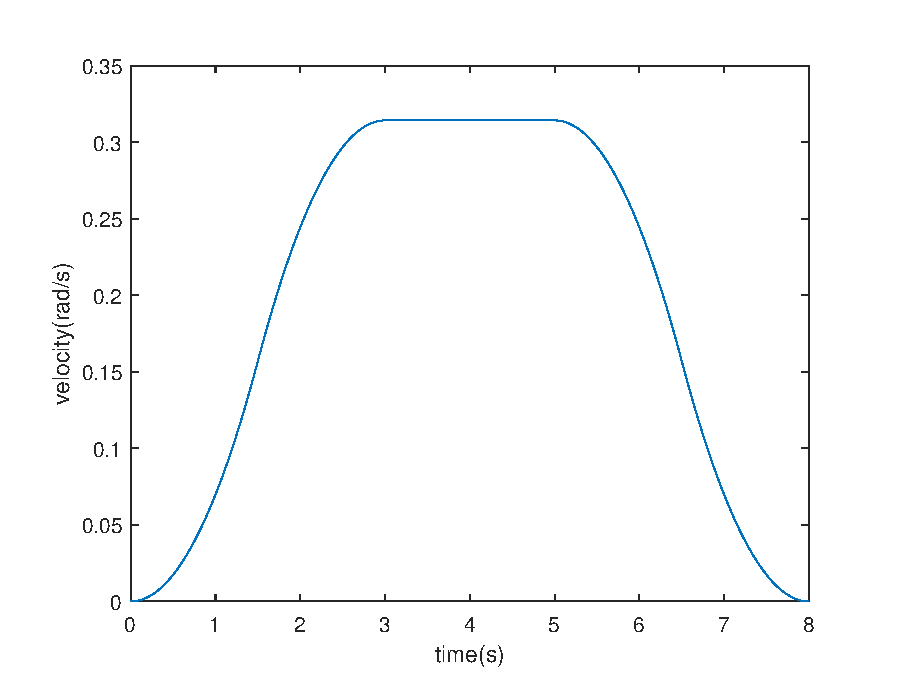
\includegraphics[width=0.45\textwidth]{Scurve}}
    \caption{Two motion profiles used in this project} 
\end{figure}
We can see that the advantage of the Trapezoidal motion profile is its simplicity and directness, with relatively simple calculations and easy implementation. However, its disadvantage lies in the rapid velocity changes. At the critical points of constant velocity and acceleration/deceleration, the first derivative of velocity undergoes a sudden change, resulting in discontinuities in acceleration at these moments. This discontinuity may lead to unstable motion. On the other hand, although the S-curve motion profile involves relatively complex calculations, its advantage lies in smoother velocity changes at the critical points of constant velocity and acceleration/deceleration. The first derivative of velocity remains continuous(acceleration is a continuous value), resulting in more stable and reliable motion.


In Simulink, we'll write two velocity curves as functions, and then store the output waveforms into a signal generator. These waveforms will serve as the input signal for the controller. Here is the specific MATLAB code:
\begin{lstlisting}[language=Matlab, frame=single, rulecolor=\color{black}]
    % Trapezodial generator
    clear;
    clc;
    phi = pi / 2; % Total rotation angle(rad)
    ta = 3; % Acceleration/Deceleration time
    tm = 2; % Time running in constant speed
    
    vm = phi / (ta + tm); % Max speed
    
    cnt = 0;
    t = 0:0.01:(2 * ta + tm);
    
    for ti = 0:0.01:(2 * ta + tm)
        cnt = cnt + 1;
        if ti < 0
            v(cnt) = 0;
        elseif ti < ta
            v(cnt) = vm / ta * ti;
        elseif ti < ta + tm
            v(cnt) = vm;
        elseif ti < ta * 2 + tm
            v(cnt) = vm - vm / ta * (ti - tm - ta);
        else
            v(cnt) = 0;
        end
    end
    
    figure(1);
    plot(t, v);
    xlabel('time(s)');
    ylabel('velocity(rad/s)');

    % S-curve generator
    clear;
    clc;
    phi = pi / 2; % Total rotation angle(rad)
    ta = 3; % Acceleration/Deceleration time
    tm = 2; % Time running in constant speed

    vm = phi / (ta + tm); % Max speed

    cnt = 0;
    t = 0:0.01:(2 * ta + tm);

    for ti = 0:0.01:(2 * ta + tm)
        cnt = cnt + 1;
        if ti < ta / 2
            v(cnt) = v1(vm, ta, tm, ti);
        elseif ti < ta
            v(cnt) = v2(vm, ta, tm, ti);
        elseif ti < ta + tm
            v(cnt) = v3(vm, ta, tm, ti);
        elseif ti < ta + tm + ta / 2
            v(cnt) = v4(vm, ta, tm, ti);
        else
            v(cnt) = v5(vm, ta, tm, ti);
        end
    end

    figure(1);
    plot(t, v);
    xlabel('time(s)');
    ylabel('velocity(rad/s)');

    % First half of the acceleration curve
    function v = v1(vm, ta, tm, t)
        v = 2 * vm / ta^2 * t.^2; 
    end

    % Second half of the acceleration curve
    function v = v2(vm, ta, tm, t)
        v = vm - 2 * vm / ta^2 * (ta - t).^2; 
    end

    % Constant speed
    function v = v3(vm, ta, tm, t)
        v = vm; 
    end

    % First half of the deceleration curve
    function v = v4(vm, ta, tm, t)
        v = vm - 2 * vm / ta^2 * (t - ta - tm).^2; 
    end

    % Second half of the deceleration curve
    function v = v5(vm, ta, tm, t)
        v = 2 * vm / ta^2 * (2 * ta + tm - t).^2;
    end
\end{lstlisting}

\newpage
\section{PID controller parameter tuning}
In this section, we will discuss the PID controller tuning process. We will use the S-curve motion profile as an example.
And we will see the differences between the PID controller parameter tuning process. Besides, this section will show you
the effect of the PID controller parameter tuning and controlling ability of three PID controllers.

In motion control, the tuning process of a PID controller can be divided into several steps. First, adjust the proportional gain $K_p$ to achieve a suitable response time $T_r$ and ensure that the system's overshoot and steady-state error are within reasonable limits.Then, adjust the derivative gain $K_d$, to reduce overshoot, minimize oscillations, and make the system response more stable. Finally, adjust the integral gain $K_i$,to eliminate any potential steady-state error, making the system response more accurate.
\subsection{Tuning process of the speed PID controller}
As the simplest controller, tuning a velocity PID controller is relatively straightforward. You can follow the parameter tuning process mentioned above to tune it. During simulation tuning, we typically start by adjusting the proportional parameter $K_p$,Below are the velocity response characteristics of the motor for different $K_p$ values.

\begin{figure}[H]
    \centering  
    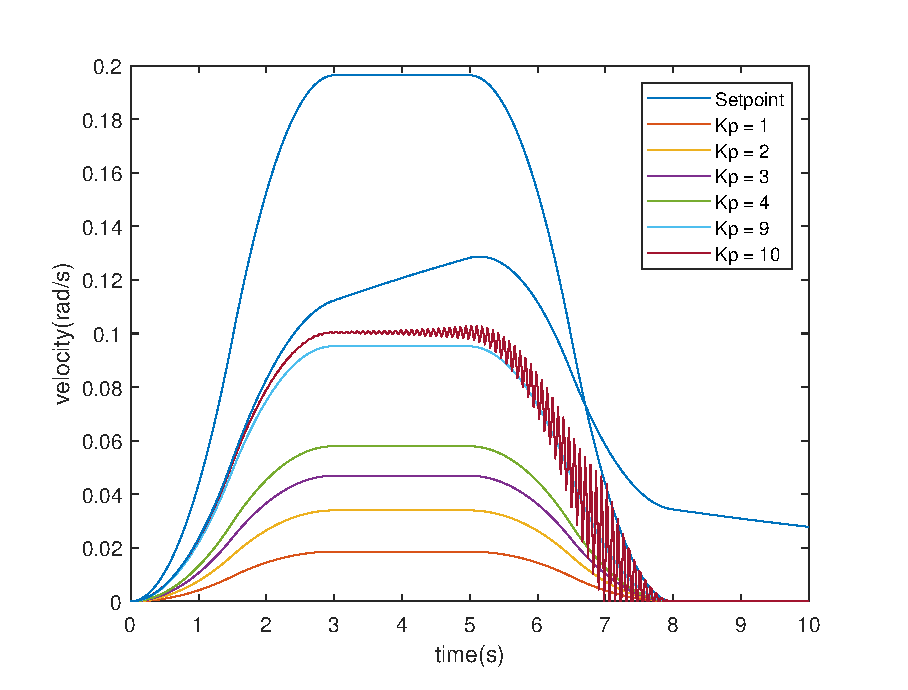
\includegraphics[width=0.8\textwidth]{SpeedKp}
    \caption{Speed response of the speed PID controller with different $K_p$}
    \label{SpeedKp}
\end{figure}
We can observe that when the value of $K_p$is small, the motor's velocity response is sluggish, and there is a large steady-state error. As $K_p$ increases, the steady-state error gradually decreases. However, when $K_p$ exceeds 10, the system response starts to oscillate, indicating instability. 
At this point, significant steady-state error still exists. Therefore, we will fix $K_p=9.5$ at 9.5 and consider trying to further reduce the steady-state error by adjusting the integral gain $K_i$.

\begin{figure}[H]
    \centering  
    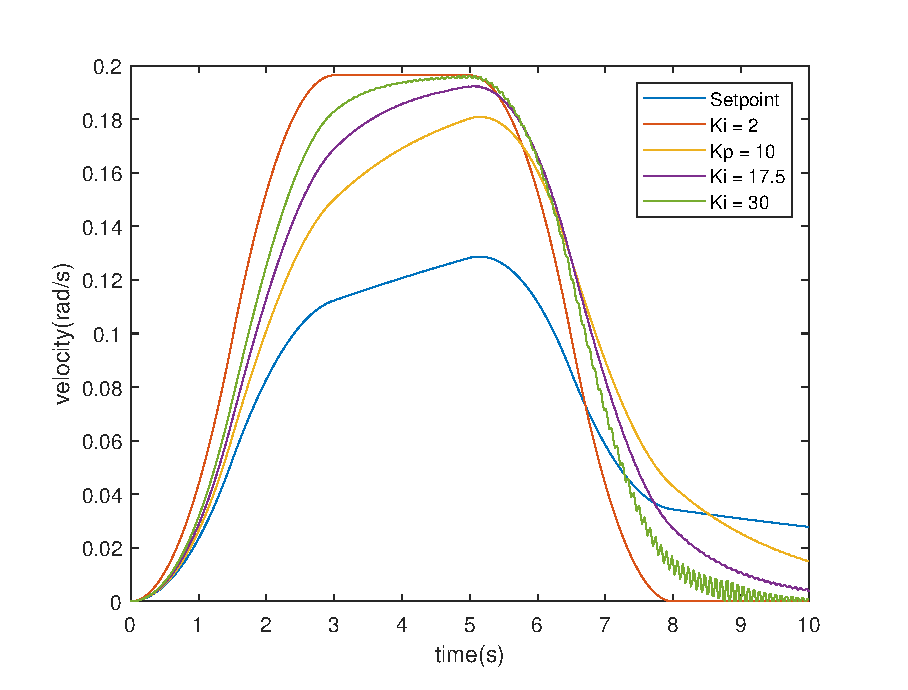
\includegraphics[width=0.8\textwidth]{SpeedKi}
    \caption{Speed response of the speed PID controller with different $K_i$($K_p=9.5$)}
    \label{SpeedKi}
\end{figure}
Similarly, when the value of $K_i$ is small, there is a large steady-state error in the system. As $K_i$ increases, the steady-state error gradually decreases. However, increasing $K_i$ further can lead to system instability. During the tuning process, it was found that when $K_i=17.75$, the overall performance is the best. However, observing the response curve as shown in Figure \ref{SpeedKi}, the system's response time is still too long, failing to reach the steady-state velocity quickly enough. Increasing $K_d$ only suppresses overshoot without addressing the issue of excessive response time. In the debugging process, it was noticed that adding $K_d$ did not significantly change the system's response.

Therefore, the final adjusted parameters for S-curve motion profile are as follows:
$$K_p=9.5, K_i=17.75, K_d=0.0005$$
Similarly, the parameters obtained for the Trapezoidal motion profile are as follows:
$$K_p=8.25, K_i=85.5, K_d=0$$

The final tuning results for the Speed PID controller with Trapezoidal motion profile and S-curve motion profile are as follows.
\begin{figure}[H]
    \centering
    \subfigure[Trapezoidal motion profile]{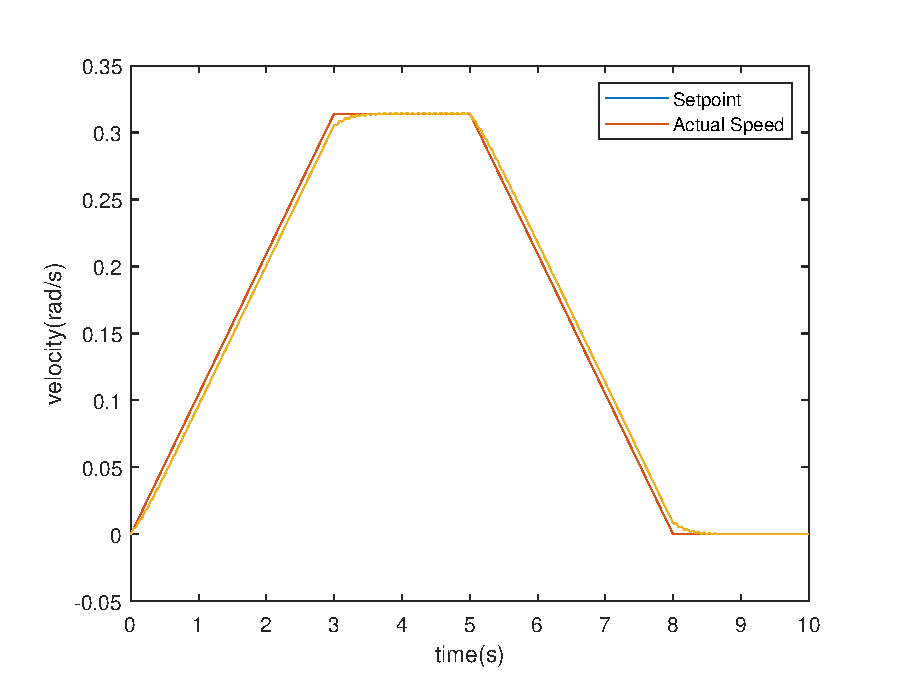
\includegraphics[width=0.45\textwidth]{SpeedKpTrapezoidal}}
    \subfigure[S-curve motion profile]{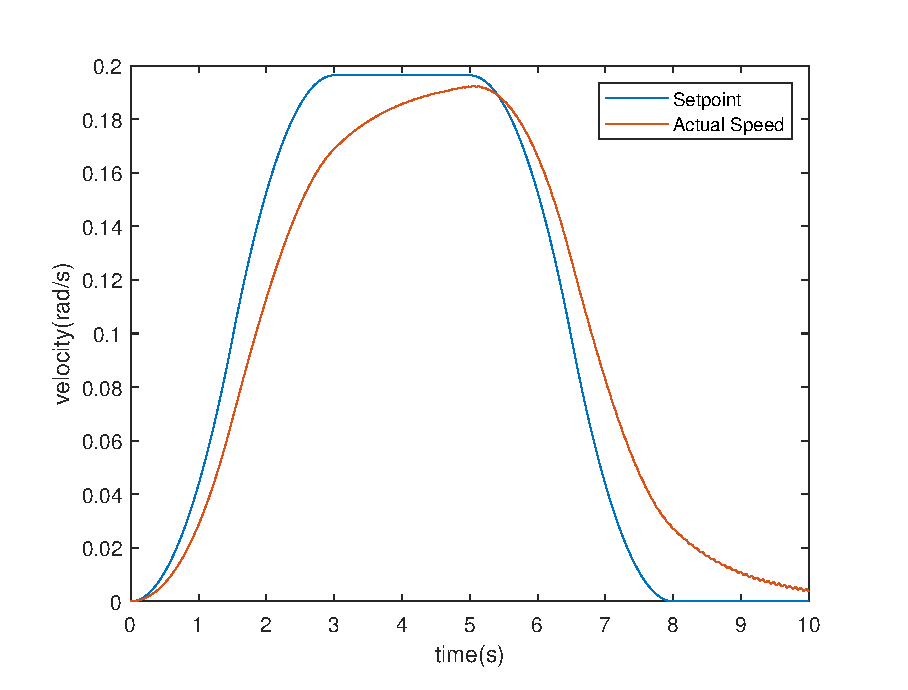
\includegraphics[width=0.45\textwidth]{SpeedKpScurve}}    
    \caption{Speed response of the speed PID controller with different motion profile}
    \label{SpeedKpMotion}
\end{figure}
We can see that for the Speed PID controller, the Trapezoidal motion profile performs better than the S-curve motion profile. Overall, the design of the Speed PID controller is relatively simple, and tuning it is straightforward. However, its control effectiveness is only moderate. In summary, its main disadvantages are:
\begin{enumerate}
    \item 
    The system's response time is relatively long, preventing it from quickly reaching the steady-state velocity in the middle.
    \item The speed of a DC motor inevitably exhibits errors, making it difficult to accurately achieve a ninety-degree angle with each displacement. In practical scenarios such as parking lots, after multiple reciprocating movements of the bar, significant drift in its range of motion will occur.
\end{enumerate}

\subsection{Tuning process of Position and velocity parallel PID controller}

During the tuning process of the Velocity PID controller, we noticed that the system's response time was too long, preventing it from quickly reaching the steady-state velocity in the middle. Therefore, we consider incorporating the position error signal for the following two reasons:
\begin{enumerate}
    \item To address the issue of excessively long system response time, which cannot be resolved by adjusting the proportional and integral gains (excessive gains leading to system instability), the addition of the position error signal aims to enable the motor to quickly reach the steady-state velocity.
    \item By monitoring the position error of the bar, we aim to resolve the issue of speed error in the DC motor, which leads to drift in the motion angle. This approach ensures that the motor can accurately move to the target position.
\end{enumerate}
In the parameter tuning process described above, we found that when $K_p>10$, the system becomes unstable, and the steady-state error remains significant. Therefore, we consider adjusting the gain of the Position Loop to reduce the steady-state error of the system and enable it to reach the steady-state velocity in the middle more quickly. Firstly, we fix the proportional gain $K_p$ in the Velocity Loop at 9. Secondly, following the tuning sequence of PID, we start by adjusting the proportional gain $K_p$ to achieve a suitable response time $T_r$ and ensure that the overshoot and steady-state error of the system are within reasonable limits. The specific process is illustrated in the following figure.

\begin{figure}[H]
    \centering
    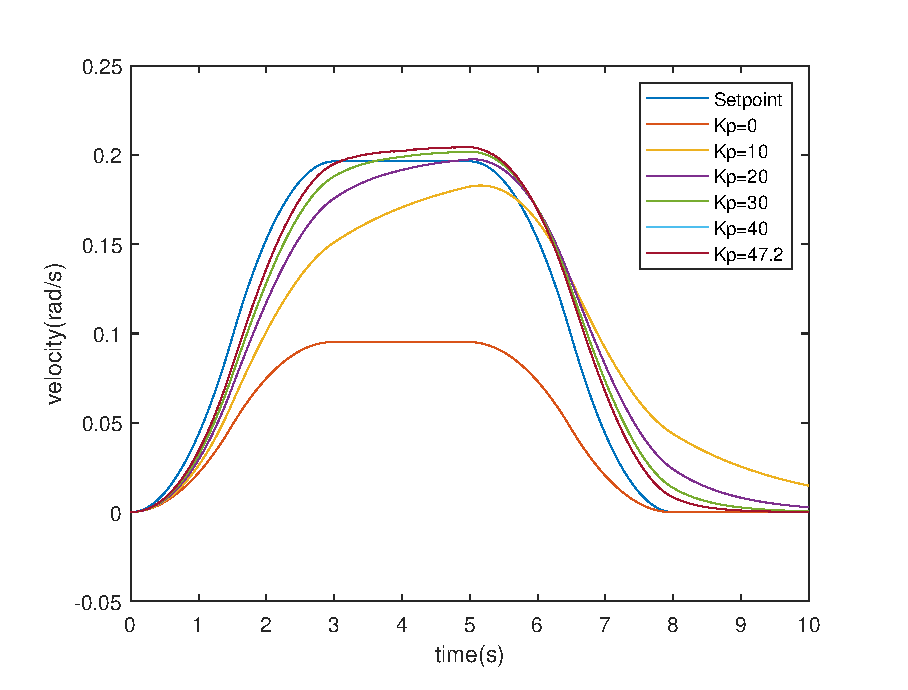
\includegraphics[width=0.8\textwidth]{2pkp}
    \caption{Speed response with different $K_p$ of position loop}
    \label{2pkp}
\end{figure}
Observing the curve in Figure \ref{2pkp}, we find that when $K_p$ is small, the system's response time is long, and it cannot quickly reach the steady-state velocity in the middle. As 
$K_p$ increases, the system's response time gradually decreases. When 
$K_p=47.2$, the overall curve is closer to the Setpoint, with no significant oscillations and only small steady-state error. Therefore, we fix $K_p=47.2$ and attempt to adjust the integral gain $K_i$ in both the Position Loop and Velocity Loop to minimize the system's steady-state error. Finally, after comprehensive optimization and debugging, we obtain the following parameters for the Position and Velocity parallel PID controller:
$$Position Loop:K_p=47.2; K_i=0.5; K_d=0$$
$$Velocity Loop:K_p=8;K_i=13.7;K_d=0$$

The final tuning results for the Speed PID controller with Trapezoidal motion profile and S-curve motion profile are as follows:
\begin{figure}[H]
    \centering
    \subfigure[Trapezoidal motion profile]{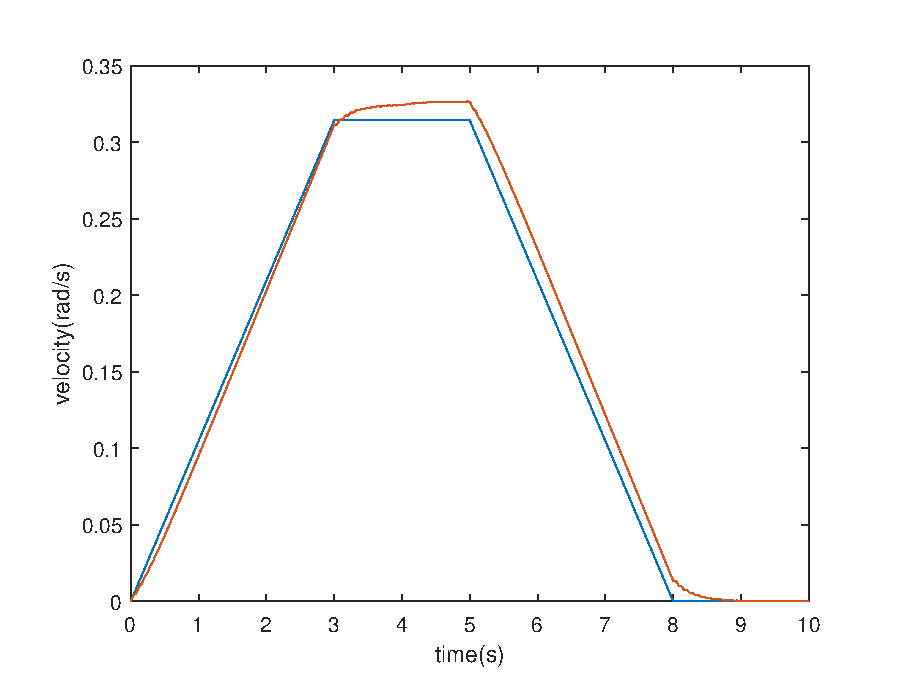
\includegraphics[width=0.45\textwidth]{2}}
    \subfigure[S-curve motion profile]{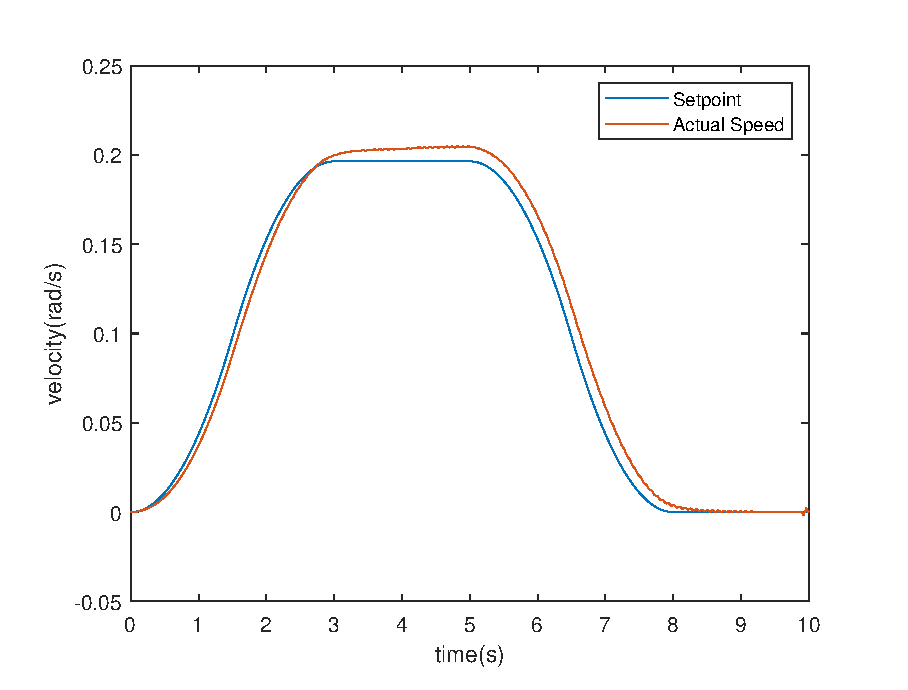
\includegraphics[width=0.45\textwidth]{1}}
    \caption{Speed response of the position and velocity parallel PID controller with different motion profile}
    \label{1}
\end{figure}
Additionally, the curve depicting the actual position versus the target position is shown in the following figure.
\begin{figure}[H]
    \centering
    \subfigure[Trapezoidal motion profile]{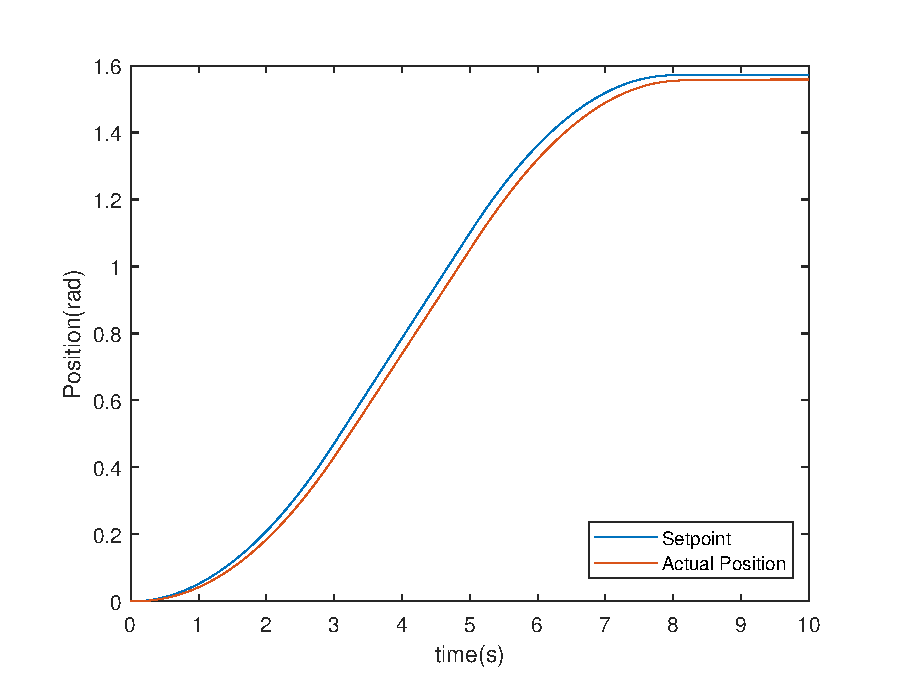
\includegraphics[width=0.45\textwidth]{3}}
    \subfigure[S-curve motion profile]{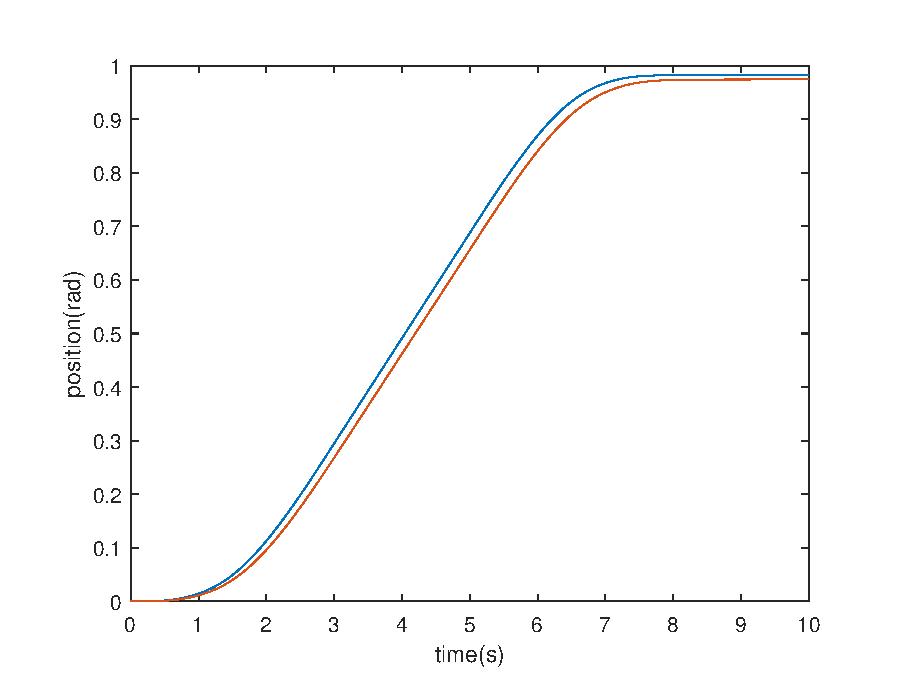
\includegraphics[width=0.45\textwidth]{4}}
    \caption{Position response of the position and velocity parallel PID controller with different motion profile}
    \label{2}
\end{figure}

You can see that for the Position and Velocity parallel PID controller, the Trapezoidal motion profile and S-curve motion profile yield similar results, with fast velocity adjustment and minimal steady-state error. Observing Figure \ref{1}, the system's velocity response curve closely follows the Setpoint, but minor curve distortions occur locally at corners. Examining Figure \ref{2}, the curve depicting actual position versus target position closely aligns, with minimal final position error, achieving precise position control as initially intended. And in our actual project, we also utilize this controller.

Overall, the design of the Position and Velocity parallel PID controller is complex, and tuning it can be challenging. However, its control effectiveness is notably good. In summary, its main advantages are:
\begin{enumerate}
    \item The system exhibits short response times, reaching the steady-state velocity quickly. Additionally, by adjusting the position error signal, it addresses speed errors in the DC motor, thereby resolving issues related to motion angle drift. Consequently, the motor can accurately reach the target position.
    \item The system maintains a small steady-state error, allowing for precise control of the motor's position. Moreover, it can swiftly reach the steady-state velocity in the middle.
    \item The system exhibits good versatility, performing well with both Trapezoidal motion profile and S-curve motion profile, indicating robustness.
\end{enumerate}

\subsection{Tuning process of Position, speed, current serial PID controller}
In engineering applications, the Position, Speed, Current serial PID controller is a commonly used controller. Its characteristic lies in its ability to simultaneously control the position, speed, and current of the motor. Engineering experience indicates that this controller yields good control effectiveness. The tuning process is similar to that of the previous PID controller, but with three closed loops for position, speed, and current. Therefore, the tuning process is more complex. Generally, starting from the innermost current loop, adjustments are made step by step, ending with the outermost position loop. The effects and tuning sequence of the three gains are similar to those of the previous PID controller. Hence, we won't delve into the tuning process of the Position, Speed, Current serial PID controller here. The final parameters are as follows:
$$Position Loop:K_p=12; K_i=0; K_d=0$$
$$Velocity Loop:K_p=0.5;K_i=283;K_d=0.006$$
$$Current Loop:K_p=0.9;K_i=0;K_d=0$$

The final control effectiveness (both speed and position control) of the controller with Trapezoidal motion profile and S-curve motion profile is as follows:
\begin{figure}[H]
    \centering
    \subfigure[Trapezoidal motion profile]{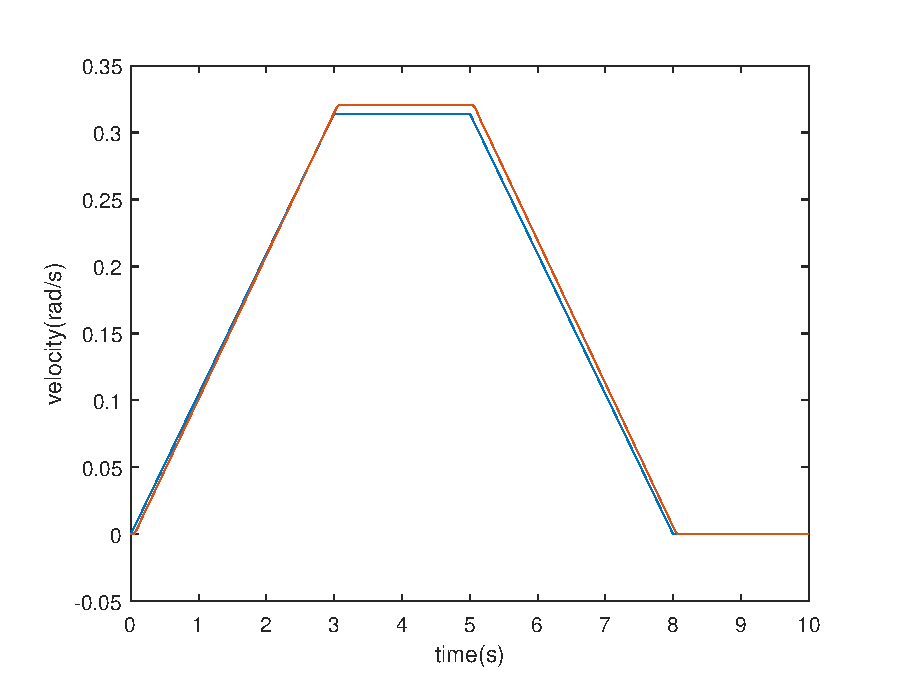
\includegraphics[width=0.45\textwidth]{5}}
    \subfigure[S-curve motion profile]{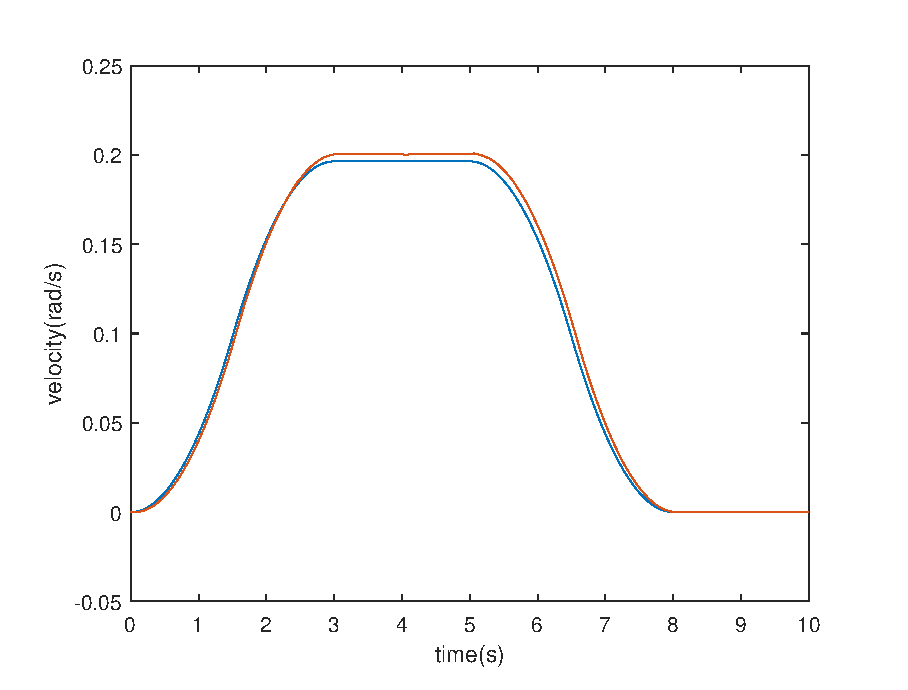
\includegraphics[width=0.45\textwidth]{6}}
    \caption{Speed response of the position, speed, current serial PID controller with different motion profile}
    \label{3}
\end{figure}
\begin{figure}[H]
    \centering
    \subfigure[Trapezoidal motion profile]{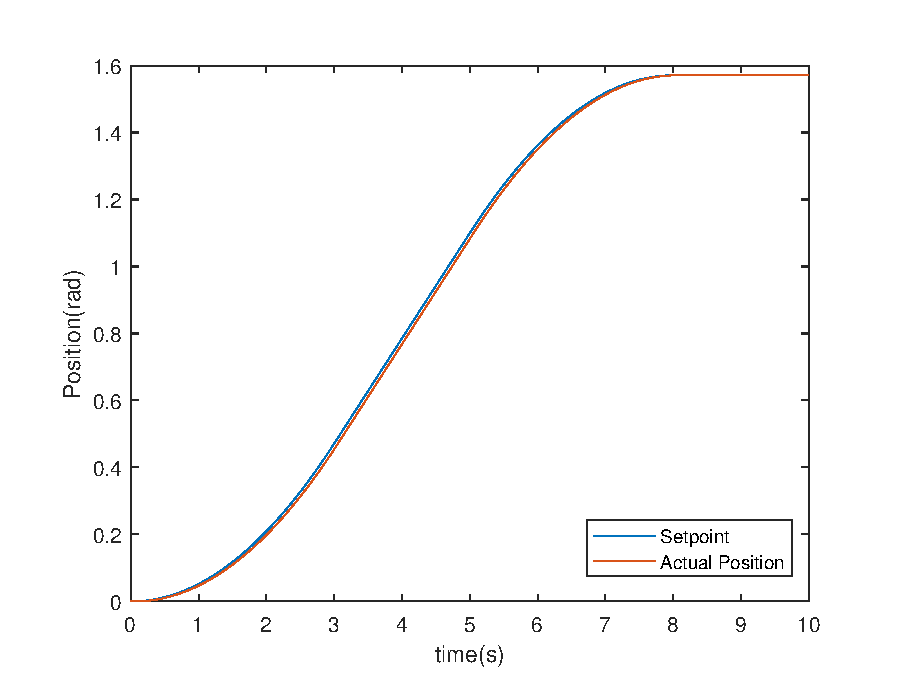
\includegraphics[width=0.45\textwidth]{7}}
    \subfigure[S-curve motion profile]{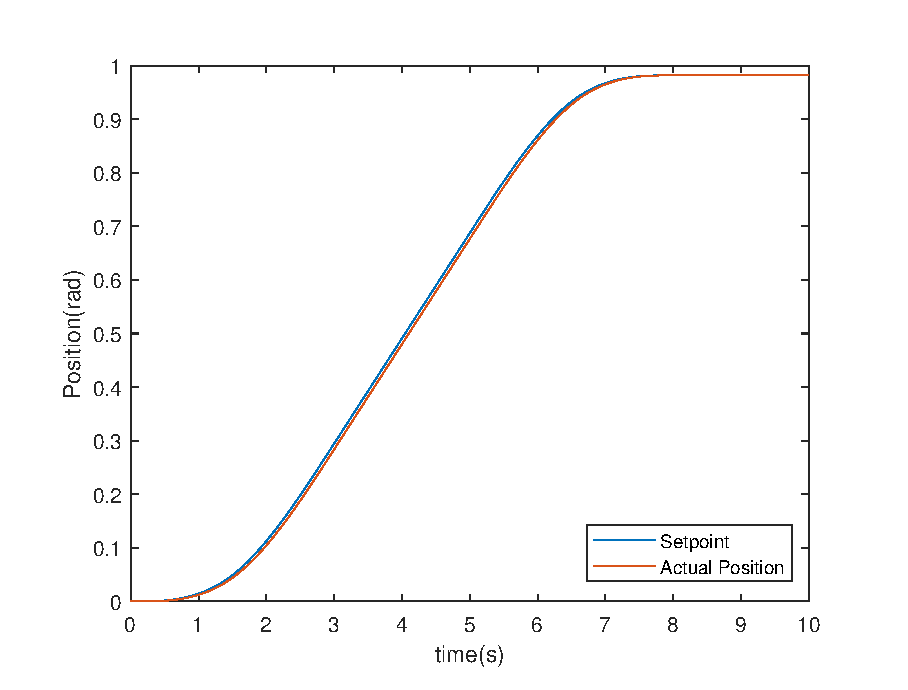
\includegraphics[width=0.45\textwidth]{8}}
    \caption{Position response of the position, speed, current serial PID controller with different motion profile}
    \label{4}
\end{figure}


It can be observed that for the Position, Speed, Current serial PID controller, both Trapezoidal motion profile and S-curve motion profile yield similar results, with excellent control effectiveness. The actual position closely matches the target position, satisfying our design goals of stability, accuracy, and safety. Overall, although the design and tuning process of the Position, Speed, Current serial PID controller are complex, its control effectiveness is notably good. It can rapidly reach steady-state velocity without oscillations and accurately control the motor's tracking target position, maintaining stability without drift issues. Therefore, it is a highly feasible and robust controller.

\subsection{Laws in the parameters of PID controller}
According to the tuning process above, we can summarize the some laws in the parameters of PID controller tuning as follows:
\begin{table}[H]
    \centering
    \caption{Parameters of PID controller}
    \label{law}
    \begin{tabular}{ccccc}
    \toprule
        \textbf{Response} & \textbf{Rise Time} & \textbf{Overshoot} & \textbf{Settling Time} & \textbf{Steady-State Error}\\
    \midrule
        $K_p$ & Decrease & Increase & NT & Decrease \\

        $K_i$ & Decrease & Increase & Increase & Eliminate \\

        $K_d$ & NT & Decrease & Decrease & NT \\
    \bottomrule
    \end{tabular}
\end{table}

\newpage
\section{System Identification}
Regarding the three PID controllers mentioned above, they have demonstrated different effects in controlling the DC motor. To further understand their characteristics, we will utilize the Matlab System Identification Toolbox for system identification in this chapter. This will help us better understand the working principles of PID controllers. We will take the Speed PID controller as an example and introduce the basic methods and steps of system identification.
\subsection{Speed PID controller}
aking the parameters of the closed-loop system concerning the S-curve as an example, we will define the input as a unit step input and the output as the step response of the motor velocity under this parameter. We will sample and save the data, with a sampling period $T_s=0.02s$。
\begin{figure}[H]
    \centering
    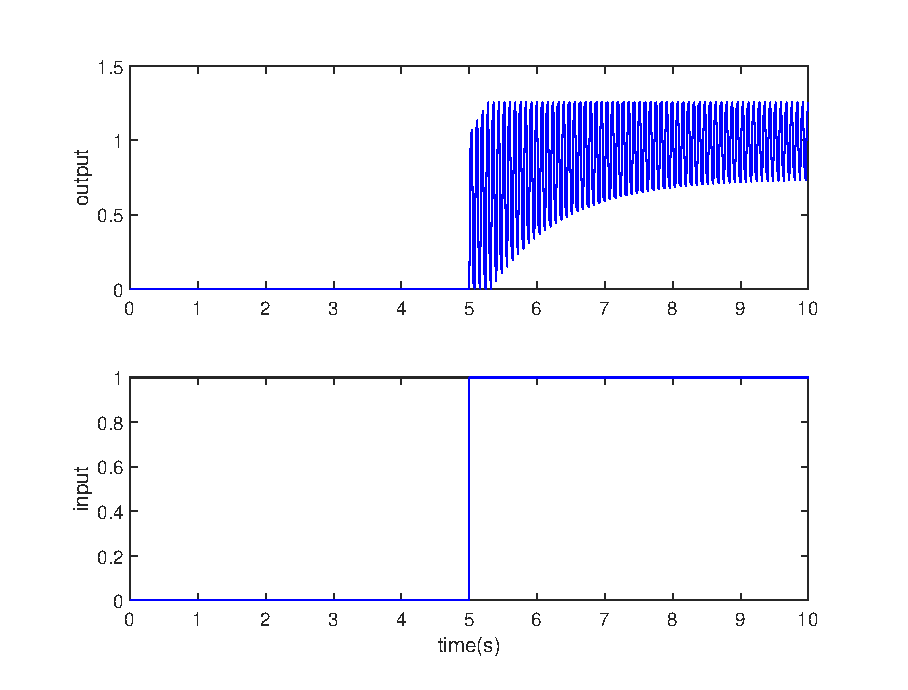
\includegraphics[width=0.8\textwidth]{inoutput}
    \caption{input and output signal}
    \label{inoutput}
\end{figure}
Import the time-domain signal into the System Identification Toolbox and set the system model to the transfer function form, as shown in the figure below.
\begin{figure}[H]
    \centering
    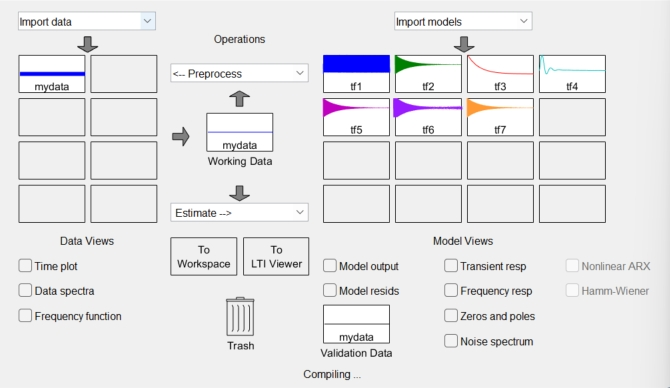
\includegraphics[width=0.8\textwidth]{tf}
    \caption{System identification}
    \label{model}
\end{figure}

Set different numbers of zeros and poles to obtain the system models on the right side of the figure, then select the optimal model and obtain the optimal parameters. The fitting degrees under different numbers of zeros and poles are shown in the table below.
\begin{table}[H]
    \centering
    \caption{Fitting degree of the system model}
    \label{degree}
    \begin{tabular}{ccc}
    \toprule
    \textbf{Number of zeros} & \textbf{Number of poles} & \textbf{Dit to estimation data} \\
    \midrule
    1 & 2 & 53\% \\
    1 & 3 & 80.12\% \\
    1 & 4 & 13.77\% \\
    1 & 5 & 51.3\% \\
    2 & 3 & 96.1\% \\
    2 & 4 & 63.46\% \\
    3 & 4 & 96.33\% \\
    \bottomrule
    \end{tabular}
\end{table}
Taking into account both the fitting degree of the data and the complexity of the system, we believe that the transfer function of the system should have 2 zeros and 3 poles. Therefore, its transfer function is as follows:
\begin{equation}
    H(s)=\frac{0.783s^2 + 1.366s + 0.04152}{s^3 + 0.02474s^2 + 2.467s + 0.04119}
\end{equation}
The zero-pole plot of the system is as shown in the figure.
\begin{figure}[H]
    \centering
    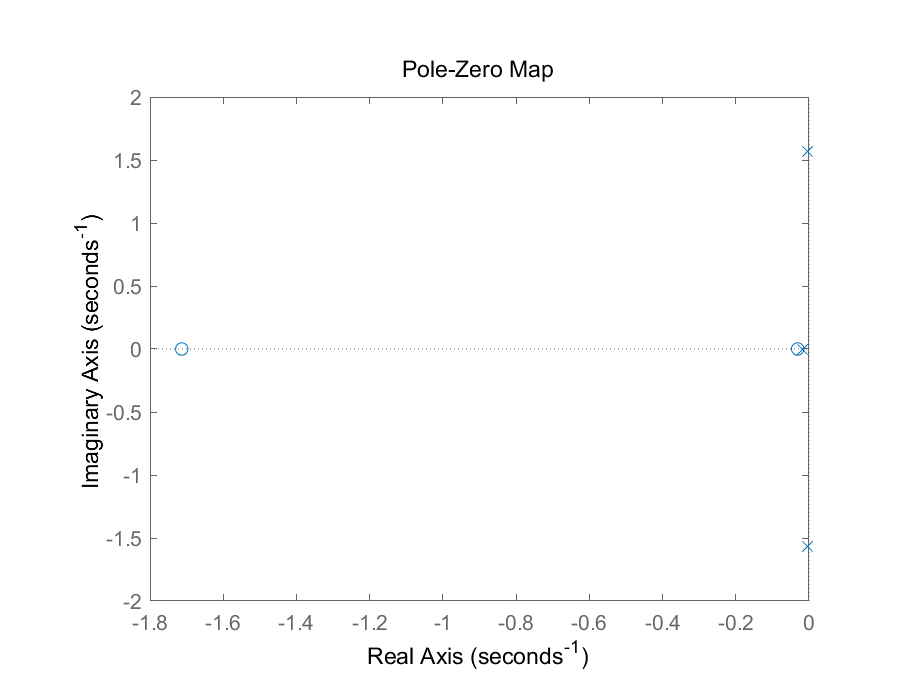
\includegraphics[width=0.7\textwidth]{zeros}
    \caption{System zero-poles diagram}
    \label{zeros}
\end{figure}
The Bode plot of the system is as shown in the figure.
\begin{figure}[H]
    \centering
    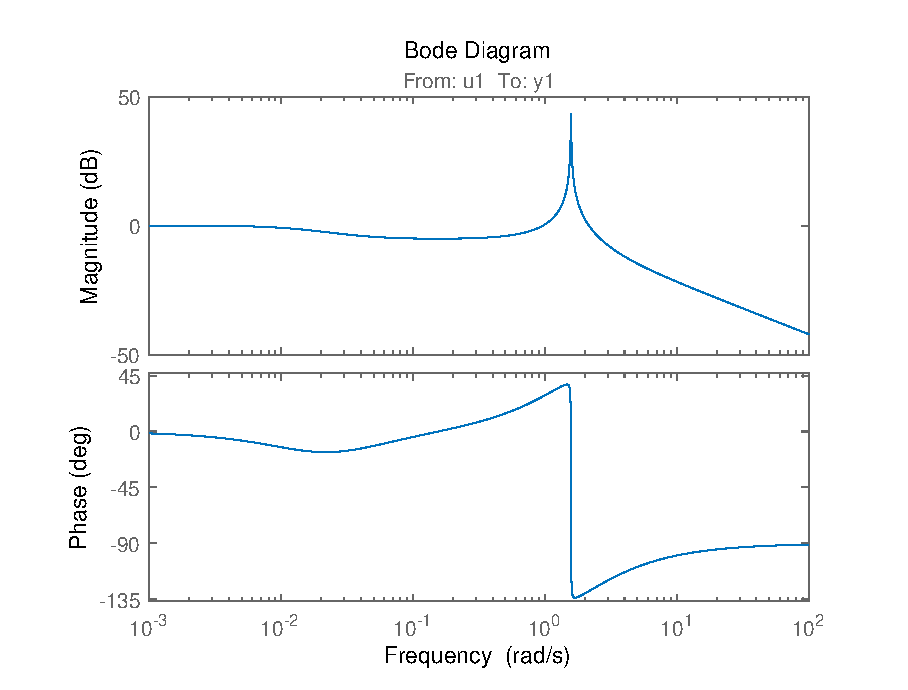
\includegraphics[width=0.8\textwidth]{bode}
    \caption{System Bode diagram}
    \label{bode}
\end{figure}
Similarly, the transfer function of the system under the parameters corresponding to the Trapezoidal curve can be obtained as follows:
\begin{equation}
    H(s)=\frac{38.14s^2 + 3150s + 3.316e04}{s^3 + 8.869s^2 + 5828s + 3.317e04}
\end{equation}
\subsection{Position and velocity parallel PID controller}
\begin{figure}[H]
    \centering
    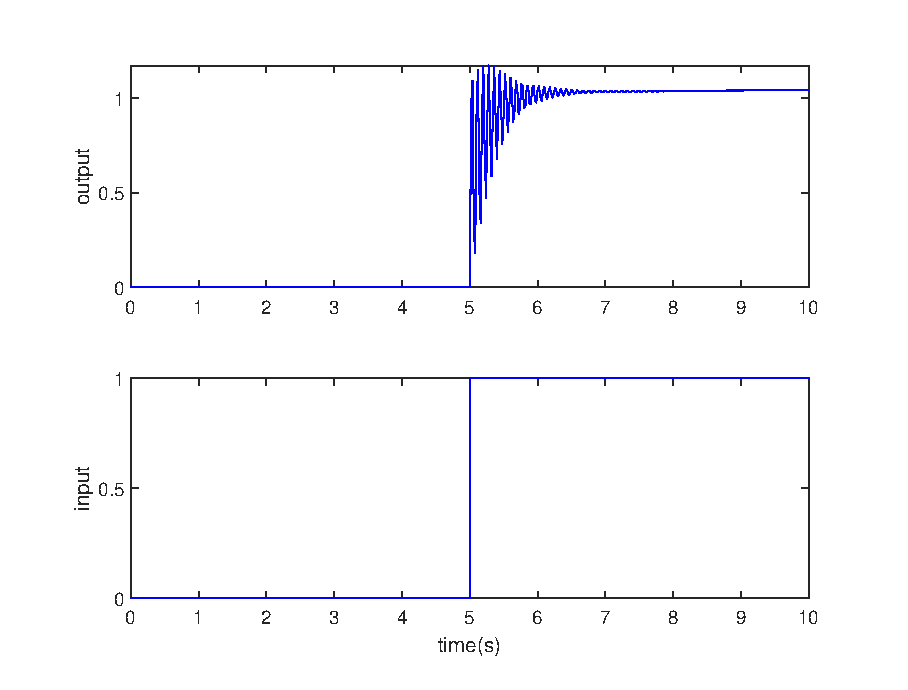
\includegraphics[width=0.8\textwidth]{abc}
    \caption{input and output signal}
    \label{inoutput}
\end{figure}
Based on the system identification method described above, the transfer function of the closed-loop system for the Position and Velocity parallel PID controller can be obtained as follows:
\begin{equation}
    H(s)=\frac{37.44s^2 + 3236s + 2.203e04}{s^3 + 8.954s^2 + 5914s + 2.126e04}
\end{equation}

\newpage
\subsection{Position, speed, current serial PID controller}
Since the input for the Position, Speed, Current serial PID controller is displacement, here we consider the system's response under ramp input.
\begin{figure}[H]
    \centering
    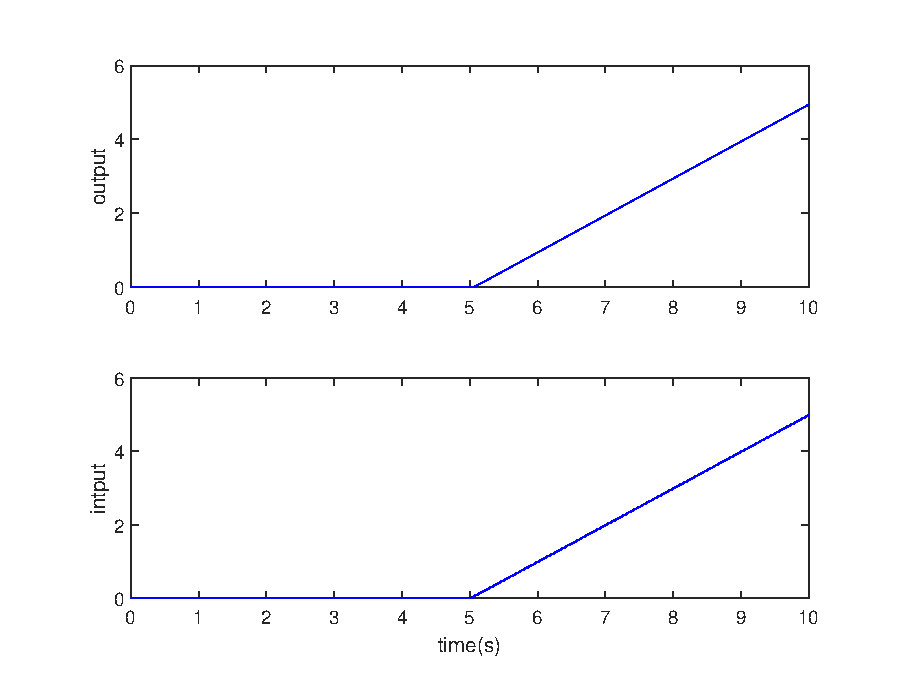
\includegraphics[width=0.8\textwidth]{asd}
    \caption{input and output signal}
    \label{inoutput}
\end{figure}
According to the aforementioned system identification method, the transfer function of the closed-loop system for the Position, Speed, Current serial PID controller can be obtained as follows:
\begin{equation}
    H(s)=\frac{-7.687s + 1638}{s^2 + 66.04s + 1638}
\end{equation}

\end{document}